\documentclass[tikz]{standalone}
\usepackage{tikz}

\begin{document}
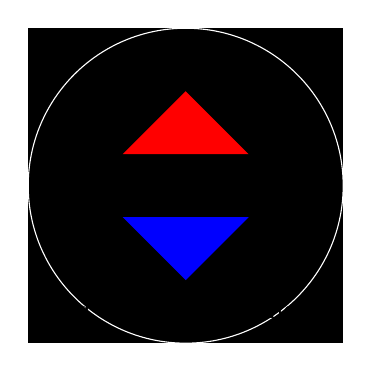
\begin{tikzpicture}[scale=2]
    % Background and Circle
    \fill[black] (-1,-1) rectangle (1,1);
    \draw[white] (0,0) circle (1);

    % Arrow Inside the Circle
    \draw[thick, ->] (0,0) -- (0.5,0);

    % Triangle Inside the Circle
    \fill[red] (0,0.6) -- (0.4,0.2) -- (-0.4,0.2) -- cycle;
    \fill[blue] (0,-0.6) -- (0.4,-0.2) -- (-0.4,-0.2) -- cycle;

    % Labels
    \node at (0,0.8) {White Circle};
    \node at (0,-0.8) {Red and Blue Triangles};
    \node at (0.7,0) {Arrow};

\end{tikzpicture}
\end{document}